% The context window grows with every turn and is re-sent whole.
% ---------------------------------------------------------------------------
% style.tex --- shared preamble for every figure in book/figures/tikz/
%
% One style for all figures: Latin Modern, thin black lines, a light grey
% fill, and one accent colour used only to mark what is untrusted or wrong.
% Build with scripts/build_figures.sh; see book/figures/README.md.
% ---------------------------------------------------------------------------
\documentclass[tikz,border=6pt]{standalone}
\usepackage[T1]{fontenc}
\usepackage{lmodern}
\usetikzlibrary{arrows.meta,positioning,shapes.geometric,calc,fit,backgrounds}

\hyphenpenalty=10000   % short lines in boxes: ragged, never hyphenated

\definecolor{lightgrey}{gray}{0.92}
\definecolor{accent}{HTML}{9B2D20}

\tikzset{
  every picture/.style={
    line width=0.6pt,
    font=\small,
    >={Stealth[length=5pt,width=4pt]},
    node distance=14pt and 24pt,
  },
  % shapes
  box/.style={draw, rectangle, inner xsep=8pt, inner ysep=5pt,
              minimum height=22pt, align=center},
  grey/.style={box, fill=lightgrey},
  rounded/.style={box, rounded corners=9pt},
  decision/.style={draw, diamond, aspect=2.4, inner sep=1.5pt, align=center},
  group/.style={draw, dashed, rounded corners=5pt, inner sep=7pt},
  % text
  tag/.style={font=\footnotesize, align=center, inner sep=2pt},
  note/.style={font=\footnotesize\itshape, align=center, inner sep=2pt},
  code/.style={font=\small\ttfamily},
  codetag/.style={font=\footnotesize\ttfamily, align=center, inner sep=2pt},
  title/.style={font=\small\scshape, align=center, inner sep=2pt},
  % lines
  arrow/.style={->},
  back/.style={->, dashed},
  thin/.style={line width=0.4pt, gray},
  % the one accent, for what is untrusted, wrong or missing
  bad/.style={accent},
  badbox/.style={box, draw=accent, text=accent},
}

\begin{document}
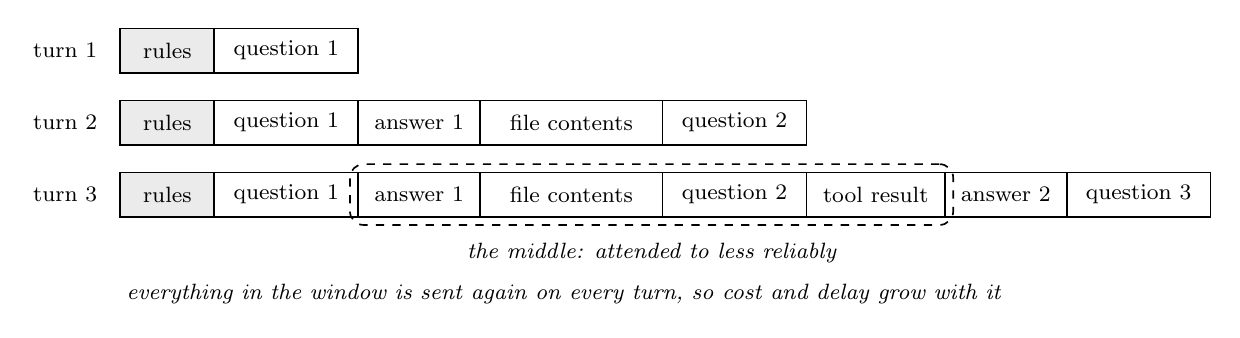
\begin{tikzpicture}[seg/.style={box, minimum height=16pt, inner sep=3pt,
                                font=\footnotesize, anchor=west, outer sep=0pt},
                    rules/.style={fill=lightgrey},
                    node distance=0pt and 0pt]
  \node[tag, anchor=east] at (-6pt,0) {turn 1};
  \node[seg, rules, minimum width=34pt] (a1) at (0,0) {rules};
  \node[seg, minimum width=52pt, right=of a1] (a2) {question 1};

  \node[tag, anchor=east] at (-6pt,-26pt) {turn 2};
  \node[seg, rules, minimum width=34pt] (b1) at (0,-26pt) {rules};
  \node[seg, minimum width=52pt, right=of b1] (b2) {question 1};
  \node[seg, minimum width=44pt, right=of b2] (b3) {answer 1};
  \node[seg, minimum width=66pt, right=of b3] (b4) {file contents};
  \node[seg, minimum width=52pt, right=of b4] (b5) {question 2};

  \node[tag, anchor=east] at (-6pt,-52pt) {turn 3};
  \node[seg, rules, minimum width=34pt] (c1) at (0,-52pt) {rules};
  \node[seg, minimum width=52pt, right=of c1] (c2) {question 1};
  \node[seg, minimum width=44pt, right=of c2] (c3) {answer 1};
  \node[seg, minimum width=66pt, right=of c3] (c4) {file contents};
  \node[seg, minimum width=52pt, right=of c4] (c5) {question 2};
  \node[seg, minimum width=50pt, right=of c5] (c6) {tool result};
  \node[seg, minimum width=44pt, right=of c6] (c7) {answer 2};
  \node[seg, minimum width=52pt, right=of c7] (c8) {question 3};

  \node[group, fit=(c3) (c6), inner sep=3pt] (mid) {};
  \node[note, below=4pt of mid] {the middle: attended to less reliably};
  \node[note, anchor=west] at (0pt,-88pt)
    {everything in the window is sent again on every turn, so cost and delay grow with it};
\end{tikzpicture}
\end{document}
